\documentclass[letterpaper]{sig-alternate}

\setlength{\pdfpagewidth}{\paperwidth}
\setlength{\pdfpageheight}{\paperheight}

\usepackage{amssymb}
\usepackage{t1enc}
\usepackage[latin1]{inputenc}
\usepackage{amsmath}
\usepackage{mathrsfs}
\usepackage{stmaryrd}
\usepackage{graphicx}
\usepackage{boxedminipage}
\usepackage{algpseudocode}
\usepackage{listings}
\usepackage[inline,nomargin,draft]{fixme}
\usepackage{xspace}
\usepackage{url}
\usepackage{color} 
\usepackage{enumerate}
\usepackage{mdwlist}

\lstset{language=[Sharp]C,
	captionpos=b,
	frame=lines,
	basicstyle=\ttfamily,
	commentstyle=\color{green},
	stringstyle=\color{red},
	numbers=left,
	numberstyle=\tiny,
	numbersep=5pt,
%  	breaklines=true,
	tabsize=2,
	escapeinside={(*@}{@*)},
	showstringspaces=false,
	keywords={this,double,bool,int,unsigned,char,true,false,void,public,static,string,new,for,return},
	keywordstyle=\color{blue},
	emphstyle=\color{cyan},
	morekeywords=[2]{Contract,Memory,Rsd,Tmp,DestRsd,DestTmp,BindRsd,This,Return,AddRsd,AddTmp,IterationSpace,RsdType,System,Diagnostics,Contracts,Requires,Ensures,Assume,Result},
	keywordstyle=[2]\color{blue},	emph={Contract,Memory,Rsd,Tmp,DestRsd,DestTmp,BindRsd,This,Return,AddRsd,AddTmp,IterationSpace,RsdType,System,Diagnostics,Contracts,Requires,Ensures,Assume,Result},
% 	emph={Assert,Test}, emphstyle=\color{red},
% 	emph={\using,\#define,\#ifdef,\#endif,\#region,\#endregion}, emphstyle={\color{blue}}
}

\usepackage[hyperfootnotes=true,colorlinks=true]{hyperref}

\begin{document}

\newcommand\mono[1]{\texttt{#1}} 

%
% --- Author Metadata here ---
\conferenceinfo{TOPI}{'11, May 28, 2011, Honolulu, Hawaii, USA}
\CopyrightYear{2011}
\crdata{978-1-4503-0445-0/11/05}
% --- End of Author Metadata ---

% first the title is needed
\title{Resource Usage Contracts for .NET}

\numberofauthors{1}

\author{
\alignauthor
Jonathan Tapicer, Diego Garbervetsky and Martin Rouaux\\
\affaddr{Departamento de Computaci\'{o}n, FCEyN, UBA} \\
\affaddr{Buenos Aires, Argentina}\\
\email{\{jtapicer, diegog, mrouaux\}@dc.uba.ar}
}

\maketitle

\begin{abstract}
In this paper we present an extension of the specification language of \textsc{Code Contracts} to support resource usage specifications in .NET programs. In particular, we focus on dynamic memory consumption, a resource that can be occupied and freed during program execution by a memory manager.
%To model memory reclaiming performed by garbage collectors we assume a simplified memory model where lifetime of objects can be associated to computation units such as methods. 
We propose a new set of  annotations enabling specification of both memory consumption and lifetime properties in a modular fashion.
To verify the correctness of these annotations we rely on the \textsc{Code Contracts} static verifier and a points-to analysis. 
In order to overcome some arithmetic limitations of the engine we incorporate a symbolic calculator capable of dealing with polynomial consumption.
%We also verify lifetime annotations using a points-to analysis.
%Since the presence of a garbage collector in object-oriented languages such as C\# and Java introduces an unpredictability component in the memory allocation and liberation, we use a simplified model of memory allocation based in scopes which is deterministic and overapproximates the memory consumption when using a garbage collector.
%We define a set of annotations that extend the available ones in \textsc{Code Contracts} to support memory usage specification and a set of techniques that leverage the usage of the \textsc{Code Contracts} static verifier in combination with other tools allowing us to verify the correctness of the annotations. Therefore, obtaining a certificate of the memory consumption of the program.
This approach was implemented in a tool which fully integrated with the Visual Studio tool-suite, available as an extension, providing facilities such us autocompletion and verification at build time.
\end{abstract}

\category{D.2.4}{Software Engineering}{Software/Program Verification}[Programming by contract]

\terms{Resource usage annotations, Static verification. }

\section{Problem Statement}
Design by contract~\cite{Meyer:OOP} is a programming discipline that prescribes that software designers should define formal, precise and verifiable interface specifications for software components, extending the ordinary definition of abstract data types with preconditions, postconditions and invariants.  %\cite{SpecSharp:Overview,leavens00jml} .
%\textsc{Code Contracts}~\cite{codeContracts} is a project initiated at MSR that brings the advantages of design-by-contract programming to all .NET based programming languages enabling the use of contracts without requiring a specific compiler. 
%
%Code Contracts provides a language-agnostic way to express coding assumptions in .NET programs. 
%The contracts take the form of preconditions, postconditions, and object invariants. 
% Contracts act as checked documentation of external and internal APIs and can be used to improve testing via runtime checking, enable static contract verification, and automatic documentation generation.

While there has been some success in the adoption of contracts for enforcing functional requirements and design decisions~\cite{leavens00jml,Meyer:Eiffel}, there have not been many signs of their usage to express non-functional requirements such as performance or resource utilization requirements.  
Possible causes are the inherent difficulty of writing quantitative requirements, the lack of a convenient language to express them and tool support to verify them. 
However, in many settings it is crucial to enforce the fulfillment of this kind of requirements. Certifying memory consumption is vital to ensure safety in embedded systems; understanding the number of messages sent through a network is useful to detect performance bottlenecks or reduce communication costs, etc. 
It is well known that inferring, and even checking, quantitative bounds (e.g., resource usage) is  difficult~\cite{garber08ismm}. Nevertheless, there has been noticeable progress in techniques that compute symbolic resource usage~\cite{garber08ismm, AlbertGG09} and complexity~\cite{gulwani2010reachability} upper-bounds.

\textsc{Code Contracts}~\cite{fahndrich2010embedded} is a tool that brings the advantages of design-by-contract programming to all .NET based programming languages enabling the use of contracts without requiring a specific compiler. 
The long term  goal of the work presented here is  enabling the specification of quantitative constraints such as resource usage and performance requirements in .NET applications using \textsc{Code Contracts}. 
% These contracts could be used for documentation purposes, static or dynamic checking, synthesis, optimization or even stress testing of computational demanding systems. 
% For instance, information supplied by contracts, once instantiated,  can be used to predict resource costs of a particular process just before running it or to make scheduling decisions according to the availability of a particular resource (e.g., comparing the available memory to the predicted consumption of a set of candidate processes for launching).

In this paper we focus in enforcing dynamic memory consumption contracts. 
%Memory usage 
This is a particularly challenging problem because memory footprint does not monotonically increase during program execution. For programming languages with automatic memory reclaiming mechanism (such as .NET based languages), this problem gets even more complex since memory consumption depends on the behavior of both the application and the garbage collector (GC). 
%Having solved this problem 
We believe other quantitative requirements may be computed by using a similar approach. 

We present an extension of the \textsc{Code Contracts} annotation language designed to specify the amount of memory consumed by a method. These specifications have two possible interpretations:  while they state the program ensures that a method consumes less than a particular bound, once verified, they can be interpreted as well as a precondition stating the system requires at least the amount of memory specified in order to run safely.

The proposed extension also provides means  for specifying object lifetimes needed to model object allocation and reclaiming. Roughly speaking, we distinguish \emph{temporary} objects, created by a method (or its callees) for auxiliary calculus, 
%but not longer needed when it finishes its execution 
from \emph{residual} objects that may be used by its callers and should live longer. For the latter we provide constructs to enable client methods to reclaim some of these objects.

In order to verify the annotations we rely on \textsc{Clousot}, the \textsc{Code Contracts} static verification engine. We do so by instrumenting the original program with special counters and transforming the memory assertions into equivalent standard \textsc{Code Contracts}  assertions in terms of those counters.
Some complex quantitative annotations require an arithmetic analysis that is beyond \textsc{Clousot} capabilities. To verify such  annotations we integrate the tool with the symbolic calculator \textsc{Barvinok}~\cite{clauss2009symbolic}, allowing us to verify specifications featuring polynomials.

All this work has been implemented as a Visual Studio plugin enabling static verification and run-time checks.

%\subsection*{Outline}
The paper is organized as follows: in~\S\ref{sec:annotations} we introduce a set of annotations to describe memory consumption  contracts,  objects lifetime information and iteration spaces for loops. In~\S\ref{sec:verification} we show how to transform those annotations into code and annotations supported by \textsc{Clousot}, and how we check object lifetime annotations.
In~\S\ref{sec:barvinok} we extend the checker to support polynomial constraints using \textsc{Barvinok}.
Then, in~\S\ref{sec:implementation} we present some implementation details. We conclude in~\S\ref{sec:relatedwork} and~\S\ref{sec:conclusions} discussing some related and future work.

\section{Memory usage annotations} \label{sec:annotations}
The design of the annotations language was driven by the following considerations: 
%The design if our language are driven by the following : 
\begin{itemize*}
	\item[(i)] 
	%Given that the tool extends  \textsc{Code Contracts}, the annotations should follow its same style. This characteristic will give the user the advantage of having a natural and easy integration with the IDE such as autocompletion and inline documentation.
	 The annotations should follow the style of \textsc{Code Contracts} to  give users the advantage of having a natural and easy integration with the IDE such as autocompletion and inline documentation.
	\item[(ii)] They need to provide means to specify that objects are allocated but also potentially reclaimed by the GC in a simple and modular fashion (lifetime information). 
	\item[(iii)] They should be rich enough to allow client methods to check its own 
	%consumption/object lifetime information 
	annotations
	using the callees' resource specifications without losing much precision. 
	\item[(iv)] Both quantitative and lifetime constraints have to be in terms of methods parameters and instance variables.
	\item[(v)] The mechanism to specify consumption information should  maintain certain basic encapsulation properties of  such us information hiding.
\end{itemize*}

To represent memory recycling due to GC we based our annotation language on a very simple memory model\footnote{This model is inspired in the scoped-memory management proposed for Real-Time Java~\cite{bollella00realtime}, but in this case we just used it as an over-approximation of GC behavior.} 
where annotations are used to \emph{only} quantify  objects created by the method being specified (or its callees). 
In this setting, those objects can be \emph{temporary}, used for auxiliary computation and no longer needed at the end of method execution; or \emph{residual}, meaning objects that may be used by a client method and, therefore, should live longer.
Using escape analysis terminology, temporary objects are captured by the method whereas residual objects escape its scope.

% \begin{figure}[ht!]
% 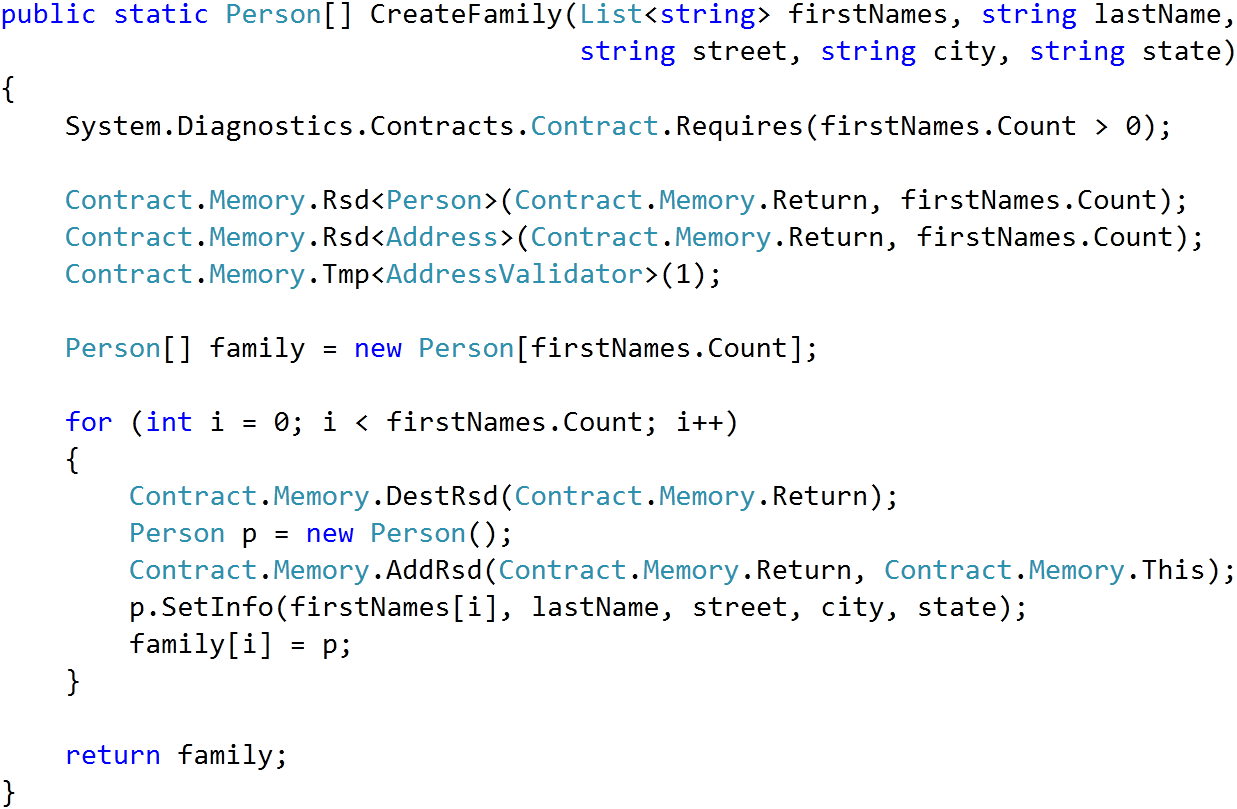
\includegraphics[width=250pt]{screen_verif_contract.png}
% %\vspace*{-2em}
% \caption{Annotated method and verification results}
% %\vspace*{-2em}
% \label{ex1}
% \end{figure}

\begin{figure}[ht]
\begin{scriptsize}
\begin{lstlisting}[numbers=none]
public Person[] CreateFamily(List<string> names,
															string address) {
	Contract.Requires(names.Count > 0);
	
	Contract.Memory.Rsd<Person[]>(Contract.Memory.Return,1); 
	Contract.Memory.Rsd<Person>(Contract.Memory.Return,
															names.Count);
	Contract.Memory.Rsd<Address>(Contract.Memory.Return,
																names.Count);
	Contract.Memory.Tmp<AddressValidator>(1);
	
	Contract.Memory.DestRsd(Contract.Memory.Return);	
	Person[] family = new Person[names.Count];

	for (int i = 0; i < names.Count; i++)	{
		Contract.Memory.DestRsd(Contract.Memory.Return);
		Person p = new Person();

		Contract.Memory.AddRsd(Contract.Memory.Return,
														Contract.Memory.This);
		p.SetInfo(names[i], address);
		family[i] = p;
	}
	return family;
}
\end{lstlisting}
\end{scriptsize}
\vspace{-1.2em}
\caption{Annotated method}
\vspace{-1.8em}
\label{ex1}
\end{figure}


Figure~\ref{ex1} shows an example exhibiting some of the annotations used to specify memory consumption. 
They are located under the \mono{Contract.Memory} class as an extension of the available class \mono{Contract} used by \textsc{Code Contracts}.

%Tmp, Rsd
\mono{Tmp} and \mono{Rsd} are used to specify  the amount  of \emph{temporal} and \emph{residual} objects consumed by a method respectively. 
%Just like the \textsc{Code Contracts} annotations \mono{Contract.Requires} and \mono{Contract.Ensures},
These annotations must be placed at the beginning of a method. They expect a class name and an integer expression which declares the number of objects of that class consumed by the method.
Notice that these annotations should be interpreted within the method as an ensures clause stating that the method consumes at most the declared number of objects, but from the client point of view its role is a requires clause demanding that the system needs at least that space for the specified quantity of objects in order to safely run. 

In addition to the quantitative expression  \mono{Rsd} expects an identifier for tagging this set of objects. The tag is used to specify that those objects belong to a group having similar characteristics in terms of lifetime (e.g., they are part of the same data structure). For instance, the identifier \mono{Contract.Memory.Return}  indicates that this set of objects is returned and  \mono{Contract.Memory.This} that objects may be reachable by the receiver. A developer can define an arbitrary set of identifiers according to hers needs of distinguishing sets of residual objects.


%DestTmp, DestRsd
To verify the aforementioned contracts we need to inform the lifetime of every object allocated by the method.  To do so, we introduce two new annotations: \mono{DestTmp} and \mono{DestRsd} which should be located before every \mono{new} statement.
\mono{DestTmp} declares that an object is temporary and \mono{DestRsd(t)} declares it as residual (living longer that the method itself) and associates the object with one of the tags already mentioned in the contract.

%AddTmp, AddRsd
In the case of method invocations we need to figure out the destination of residual objects originated in callees. 
The annotation \mono{AddTmp(src)} states that callees' residual objects tagged with \mono{src} become temporary in the caller. \mono{AddRsd(dst, src)} states that residual objects tagged with \mono{src} become residual objects identified with \mono{dst}.
%Both of them should be located before the call, in the former, the name of the \textit{residual} in the callee is required, in the later it is also required and, additionaly, the name of the local \textit{residual} that specifies the quantity of objects is also required. In Figure \ref{ex1} we can see the usage of \mono{AddRsd} that the specifies that the objects of the following call (the constructor the class \mono{Person}) that exceed the lifetime of the method through a \textit{residual} with name \mono{Contract.Memory.This} are transfered to the local \textit{residual} with name \mono{Contract.Memory.Return}.

%BindRsd
So far, we have been using tags to declare sets of residual objects. This mechanism encompasses information hiding and is sufficient to specify and enforce the quantitative aspects of method consumption. However, to check the validity of annotations concerning objects lifetime, namely \mono{DestTmp} and \mono{DestRsd}, we need to provide the checker with the means to link tags to actual objects. To do that, we introduce the annotation \mono{BindRsd(t, expr)} which connects a tag \mono{t} with a set of objects referred by the path-expression \mono{expr}.  For instance. \mono{BindRsd(List, l)} specifies the tag \mono{List} represents all objects reachable from the variable \mono{l}. 

It is worth noticing that \mono{AddTmp}, \mono{AddRsd}, \mono{DstTmp}, \mono{DstRsd} and \mono{BindRsd} are internal method annotations, not visible outside the method boundary. In contrast, \mono{Tmp}, \mono{Rsd} and their tags can used by clients.



\section{Verifying memory consumption} \label{sec:verification}
%Here we describe how to automatically check the annotations introduced in the previous section relying on \textsc{Code Contracts} verifier (\textsc{Clousot}). 
%
%Basically, we transform the annotated program into a functionally equivalent but instrumented in such way that the \textsc{Code Contracts} verifier is able to determine the correctness of the annotations.
To automatically check the annotations introduced in the previous section we transform the annotated program into a functionally equivalent program but instrumented into one using only \textsc{Code Contracts} annotations in such way  that a successful  verification of the transformed program implies the correctness of the original resource usage annotations.

\subsection{Introducing counters and ensure clauses}
%For verification purposes we will interpret the memory consumption annotations as ensures clauses. 
%The idea behind the counters and contracts instrumentation is to generate a set of counters (integer attributes in the method's class) that are incremented in the body of the method being instrumented and a transformation of the given memory contracts into \textsc{Code Contracts} native contracts so that the given assertions are expressed in function of the counters and can be verified by \textsc{Code Contracts}.
For every method \mono{m} featuring memory consumption we apply the following procedure:
let $T$ be the set of memory lifetime tags appearing in the contract (including one for temporary consumption) and $C$ the set of classes. For each tag $\mono{t} \in T$ and $\mono{C} \in C$ we introduce a counter \mono{C\_m\_t}   which tracks the number of objects  of type \mono{C}  from \mono{m}  that are associated with tag \mono{t}.
To keep the counters updated, for each  \mono{new C()} statement annotated with \mono{DestTmp} or \mono{DestRsd(t)}, we introduce a statement to increment  \mono{C\_m\_t}. 
Finally, the memory consumption annotations are transformed into corresponding ensure clauses stating that the associated counters are less than or equal to the specified bounds. 

Concretely:  \mono{Contract<C>.Rsd(t, e)} is transformed into \mono{Contract.Ensures(\mono{C\_m\_t} <= e)}. The same approach applies for  temporary consumption contracts.

%For each contract we will generate a counter, this counter will be incremented for each \textit{new} statement annotated with \mono{DestTmp} or \mono{DestRsd} where the destination of the object is the type of memory corresponding to the contract being instrumented. Then, the contract is transformed into a \mono{Contract.Ensures} annotation with an expression combining the counter and the integer expression given by the user.

% Lets see an example of this instrumentation. Given this simple method:
% 
% \vspace*{5pt}
% \begin{scriptsize}
% \begin{lstlisting}[caption=Example method not instrumented]
% public Person CreatePerson(string name)
% {
% 	Contract.Memory.Rsd<Person>(Contract.Memory.Return, 1);
% 	Contract.Memory.DestRsd(Contract.Memory.Return);
% 	return new Person(name);
% }
% \end{lstlisting}
% \end{scriptsize}
% \vspace*{5pt}
% 
% This is the same method instrumented:
% 
\begin{figure}[b]
%\vspace{1em}
 \begin{scriptsize}
 \begin{lstlisting}[numbers=none]
 public static int Person_CP_rsd_return;
 public Person CreatePerson(string name)  {
 	...
	Contract.Ensures(Person_rsd_return <= names.Count);
 	Person_CP_rsd_return = 0;
 	...		
	for (int i = 0; i < names.Count; i++)	{
		Person_CP_rsd_return++;
		Person p = new Person();
		Person_CP_rsd_return += Person_SI_this;
		p.SetInfo(names[i], address);
		...
 \end{lstlisting}
 \end{scriptsize}
 \vspace{-.5em}
\caption{Fragment of an instrumented version} \label{ex1-inst}
\end{figure}
% 
% With this instrumented code, the \textsc{Code Contracts} static verifier is going to try to verify the correctnes of the inserted contracts in line 5 and the result can be seen in the Visual Studio verification results along the \textsc{Code Contracts} results like Figure \ref{ex1} shows.

For the annotations \mono{AddTmp(d)} and \mono{AddRsd(d, s)} the instrumentation consists in adding to the respective local counters the value of the callee counter. 
%That way, \textsc{Code Contracts} will be able to determine the quantity of objects transferred from the callee using the instrumented contract the called method.

% Like we mentioned before, the \textit{temporal} memory of the called methods should be maximized and considered part of the required \textit{temporal} memory of the caller method for it to be safely executed. This is also done during the instrumentation phase using the method \mono{Math.Max} when adding to the counters, taking special care if it is done inside a loop.

The instrumentation is performed at the IL level and is never read or manipulated by developers.
Only for demonstration purposes, in Figure~\ref{ex1-inst} we show a fragment of the instrumented version of the  method presented in Figure~\ref{ex1}.

%For demonstration purposes, in Figure~\ref{ex1-inst} we show a fragment of the instrumented version of the  method presented in Figure~\ref{ex1}. Actually, the instrumentation is performed at the IL level and is never read or manipulated by developers.

\subsection{Verifying object lifetime annotations}
The instrumentation and verification process assume that object lifetime annotations \mono{DestTmp} and \mono{DestRsd} are correct. To ensure they actually are, we include a lifetime-annotations checker. 
Figure~\ref{ex2} shows an example where an escaping object is incorrectly declared as temporary. The squiggly highlights the position of that error.



To perform this verification we rely on a points-to and escape analysis capable of analyzing .NET programs~\cite{garber07iwaco}.  For every annotated method we run the analysis and build a points-to graph (PTG) which is basically an abstraction of the program heap visible from each method at the end of its  execution. To verify the correctness of \mono{DestTmp} annotation, we check whether the node in the PTG, representing objects created at that program point, is not reachable from the global scope, method parameters or the returned object.  For \mono{DestRsd} we check if the object escapes and it is reachable through the path expression associated with the tag (i.e.,  by using \mono{BindRsd}).
The correctness of the lifetime information associated to the annotations \mono{AddTmp} and \mono{AddRsd}, where the objects are transferred to the objects designated by the corresponding tags, is also verified in a similar fashion.

%Using an implementation of the algorithms defined in \cite{garber07iwaco} we do a points-to and escape analysis of the code and verify the correctness of the annotations \mono{DestTmp} and \mono{DestRsd}. 
\begin{figure}[tb]
% \fbox{
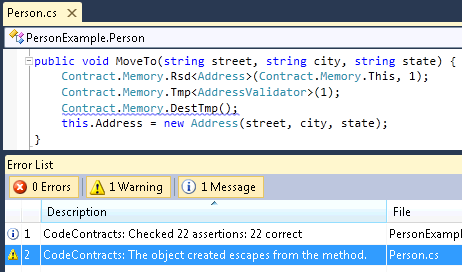
\includegraphics[width=1\linewidth, clip]{screen_verif_dest2.png}
%}
%\vspace*{-2em}
\vspace{-2em}
\caption{Lifetime annotations verification result}
\vspace*{-1em}
\label{ex2}
\end{figure}



\section{Verifying complex contracts} \label{sec:barvinok}
\textsc{Clousot} does a very good job in performing automatic verification of contracts, being able to check method featuring loops without demanding loop invariants. 
However, it has some limitations when dealing with the complex arithmetic required for a quantitative analysis. According to our experiments the current version of \textsc{Clousot} is restrained to contracts having linear integer expressions.
 %Another limitation found in the verification using \textsc{Clousot} is related to the usage of \mono{Math.Max}.} Just like with the contracts, the arithmetic module isn't able to handle non-linear expressions.

\textsc{Barvinok}~\cite{clauss2009symbolic} is a tool\footnote{\small Available at: \url{http://freshmeat.net/projects/barvinok}.} capable of manipulating parametric integer sets and relations.  It provides functionality to \emph{count} the number of elements of these sets and for performing \emph{maximization} and \emph{sum} on polynomials over these sets. 
Given a method featuring a loop (with possible several nested loops) including a \mono{new} statement  
and a predicate describing its iteration space (i.e. a linear restriction describing the relation between the loop inductive variables and parameters),  we can obtain a parametric upper-bound of the number of times the  \mono{new} statement is executed. This upper bound is obtained by counting the number of solutions of that iteration space~\cite{garber08ismm}. 
In a similar fashion, we can deal with polynomial temporary and residual consumptions by applying respectively a symbolic maximization and sum operations over the iteration space. 



For those methods whose consumption is beyond the capabilities of \textsc{Clousot} we can use this approach. The price to pay to obtain more precision is the need of a new annotation to specify iteration spaces inside loops: \mono{IterationSpace}. Although this increases the annotation burden,  the gain is considerable since it makes possible the verification (and inference) of polynomial consumption. 
Notice that iteration spaces are a set of linear constraints, amenable to  be checked with \textsc{Code Contracts} as well.
We think it will be possible to automatically generate these annotations leveraging  on \textsc{Clousot} abilities on inferring loop invariants.

\begin{figure}[hbt]
\begin{scriptsize}
\begin{lstlisting}
public List<Person> CreateBigFamily(int n) {
	Contract.Requires(n > 0);
	Contract.Memory.Rsd<Person>(Contract.Memory.Return,
															n*(n+1)/2);

	List<Person> family = new List<Person>(n*(n+1)/2);
	for (int i = 1; i <= n; i++) {
		Contract.Memory.IterationSpace(1 <= i && i <= n);
		for (int j = 1; j <= i; j++) {
			Contract.Memory.IterationSpace(1 <= j && j <= i);
			Contract.Memory.DestRsd(Contract.Memory.Return);
			Person p = new Person(); (*@ \label{ex3:new-2loop} @*)
			family.Add(p);
		}
	}
	return family;
}
\end{lstlisting}
\end{scriptsize}
\vspace{-.5em}
\caption{Using \mono{IterationSpace} to assist the prover}
\vspace{-1.5em}
\label{ex3}
\end{figure}

Figure \ref{ex3} shows a method with a loop and a nested loop inside it. In this case \textsc{Clousot} would not be able to verify the contract. 
However, using  \textsc{Barvinok} and the aid of  \mono{IterationSpace} annotations in the loops we can determine the exact number of times that the \mono{new} statement on line~\ref{ex3:new-2loop} is executed and instruct the engine with new knowledge.


%When methods get longer they tend to have several increments to the counters, and in that cases even if we always add to the counters pre-calculated expressions, the verifier isn't able to determine that the sum of all the expressions meets the contract. For these cases, we can also use \textsc{Barvinok} to help during the verification. We build an expression composed of all the expressions added to a counter and verify, using \textsc{Barvinok}, if this expression meets the given contract; if it does we give that information to the verifier introducing a \mono{Contract.Assume} statement, therefore adding this information to the verifier knowledge base and letting it verify the correctness of the contract.

\section{Implementation details} \label{sec:implementation}

% The \textsc{Code Contracts} static verifier is invoked by Visual Studio after each compilation. In order to do the instrumentation and let verifier analyze the transformed contracts we need to do it before it reaches the static verifier. This is done modifying the \textsc{Code Contracts} configuration replacing the static verifier with a modified version that does the required instrumentation and then invokes the original verifier.
% 
% \begin{figure}[ht!]
% \begin{center}
% 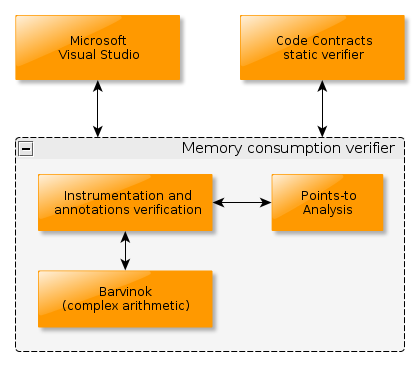
\includegraphics[scale=0.5]{arq.png}
% \end{center}
% %\vspace*{-2em}
% \caption{General architecture of the tool}
% %\vspace*{-1em}
% \label{arq}
% \end{figure}
% 
% Figure \ref{arq} shows the general architecture of the tool. The component labeled \textit{Memory consumption verifier} has the same interface as the \textsc{Code Contracts} verifier, so it can replace it when Visual Studio invokes it. Internally, the \textit{Memory consumption verifier} uses the described algorithms and tools to do the instrumentation and verification, then it invokes the \textsc{Code Contracts} verifier and returns to Visual Studio the verification results.

We developed a Visual Studio extension\footnote{\small Available at: \url{http://lafhis.dc.uba.ar/resourcecontracts}.} that lets developers write memory consumption contracts as  they do with \textsc{Code Contracts} and verify them using its static verifier or run-time checker.
The only prerequisite for the plug-in is having \textsc{Code Contracts} installed, all the other tools used by the memory contracts checker are packaged in the plugin.
We use the Common Compiler Infrastructure (CCI)~\cite{CCI} for code analysis and instrumentation.
%Memory contracts checking can be activated or deactivated in a per-project basis. 
%Once enabled, the memory contracts annotations become available in the project, having autocompletion and inline documentation, just like \textsc{Code Contracts} annotations.

The \textsc{Code Contracts} static checker is invoked by Visual Studio after each compilation. 
In order to transform the code before checking it, we use a wrapper that performs the required instrumentation and then invokes the actual checker. When the plug-in is installed it modifies the \textsc{Code Contracts} configuration in order to setup this wrapper. So far, we have not found a better way to ensure that our tool is invoked before the \textsc{Code Contracts} checker.



\section{Related work} \label{sec:relatedwork}
%Separar inferencia de verificacion. 
%Foco en memoria quizas y mas en verificacion y en herramientas existentes.
Recently, there were relevant advances in resource analysis for imperative and functional programs~\cite{chin05SAS,BarthePS05,garber08ismm,AlbertGG09,he2009memory,gulwani2010reachability,hoffmann2010amortized}.
For lack of space we will  briefly refer to some of them which are focused in verification of annotated programs. 

The work in~\cite{chin05SAS}  proposes a type system to statically check linear size annotations (Presburger's formulas) in a functional fragment of a Java-like language. This approach allows  specifications of the number of preexistent objects released  by a method but it requires  complex aliasing annotations. We prefer a coarse grained approach demanding less and easier to infer annotations.

Closer to our approach,~\cite{BarthePS05} defines an annotation language based on JML that can be used to annotate Java bytecode. This language is limited and does not contemplate the specification of lifetime information. In~\cite{he2009memory} the authors present a verification system for C-like programs using recursion as the only iteration mechanism. Similar to ours they use contracts and program instrumentation techniques using a non-specialized verifier. Their system supports \mono{free} statements which in principle enables a more precise reasoning. However, according to our experience, verifying non-linear consumption in those systems is extremely hard because of the need of machinery capable of dealing with lower and upper bounds. 

\section{Conclusions and Future Work} \label{sec:conclusions}
In this work we presented an extension of  \textsc{Code Contracts} language to specify and verify the memory consumption of .NET programs. %where memory is a critical resource, obtaining with the verification a certificate that the program will never exceed a certain parametric memory usage. 
The tool integrates with Visual Studio enabling autocompletion, inline documentation, static verification and run-time checking as \textsc{Code Contracts} does. 

As a future work, we would like to enhance the usability of the tool by automatically inferring quantitative and lifetime annotations.
In this setting developers would only need to specify complex or hard-to-infer annotations, not worrying about annotations that can be easily inferred. In this matter we plan to port our previous work on inference of memory consumption for Java~\cite{garber08ismm} to .NET and extend other tools capable of inferring resource usage (e.g.,~\cite{gulwani2010reachability}) in order to make them capable of dealing with dynamic memory usage.


\bibliographystyle{plain} % plainnat
\bibliography{garbervetsky}

\end{document}
